\newprob{lq1}{
    某種塑膠的折射率是 2.5。\\The reflective index of certain plastic is 2.5.
    \begin{parts}
        \part 計算光線從塑膠射至空氣時的臨界角。\\Calculate the critical angle when the light ray travels from plastic to air.\zh{2}
        \dlines{2}
        \part 潛望鏡 P 和 Q 以 $45^\circ-90^\circ-45^\circ$ 的塑膠塊(折射率= 2.5)如圖放置而製成。\\The periscope P and Q are made by placing two plastic blocks (refractive index = 2.5) in a $45^\circ-90^\circ-45^\circ$ configuration, as shown in the diagram.
            {\par\centering
                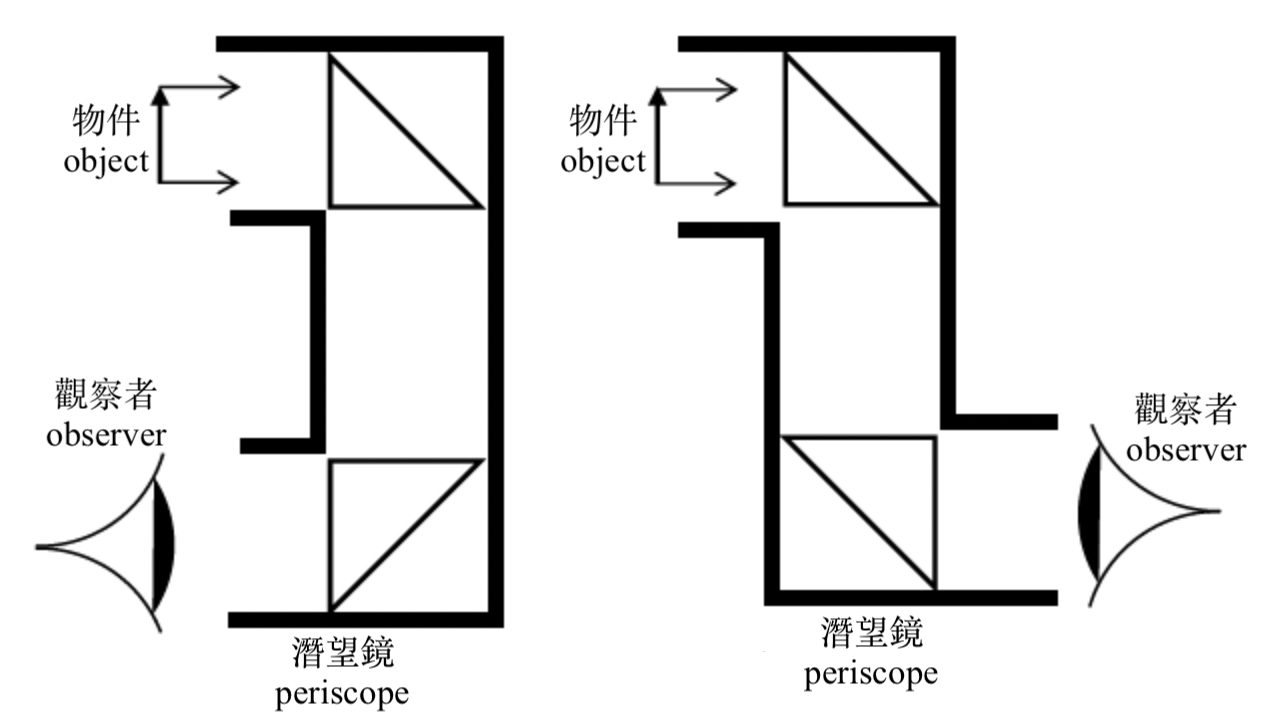
\includegraphics[width=0.85\linewidth]{latexnd89xd.png}\par}
        \part 完成圖中物件射出的光線的光路,並指出哪個潛望鏡會產生倒置的成像。\\Complete the light path of the rays emitted from the object in the diagram, and indicate which periscope will produce an inverted image.\zh{3}
        \ddlines{0.5}
        \clearpage
        \part 現有一塊 $30^\circ-60^\circ-90^\circ$ 的透明三角柱體,它的折射率為 2.5。\\Here is a transparent triangular prism with angles of $30^\circ-60^\circ-90^\circ$, and its refractive index is 2.5.
            {\par\centering
                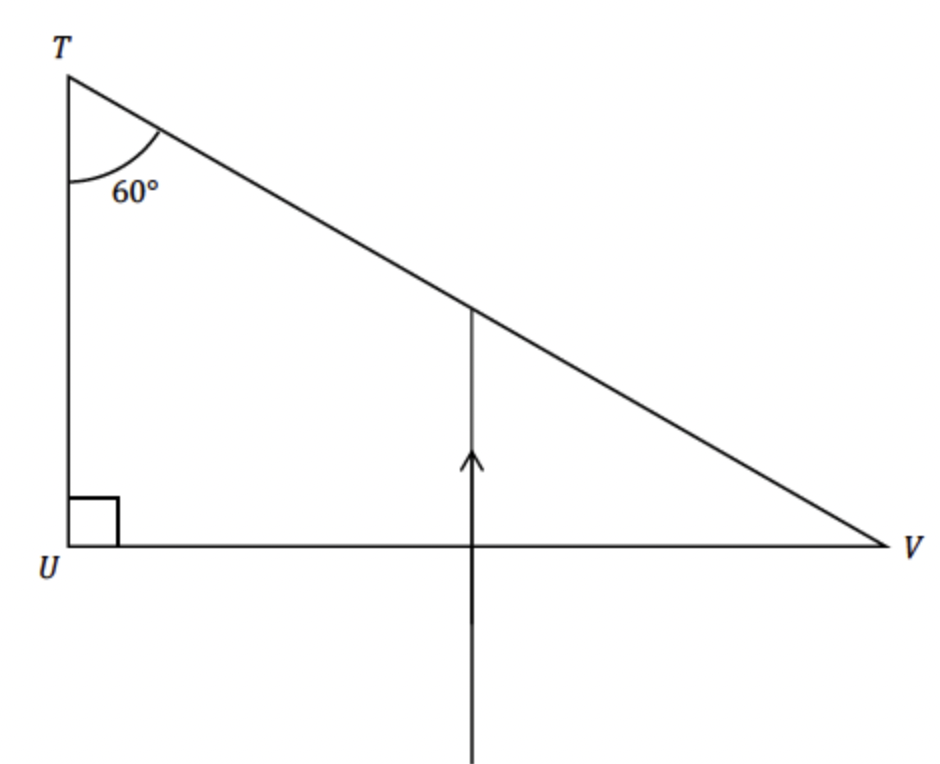
\includegraphics[width=0.5\linewidth]{92d8nud8n92c3.png}\par}\bigskip
        寫出光線首次抵達 UT 時的入射角,並以此解釋為何這柱體不適用於潛望鏡。\\Write down the angle of incidence when the light ray first reaches UT, and explain why this prism is not suitable for a periscope.\zh{2}
        \dlines{2}
    \end{parts}
}{}


\newprob{lq3}{
    細閱以下關於彩虹的文章,並回答隨後的問題。\\Read the following article about rainbows and answer the following questions.
    \begin{tcolorbox}[colback=white]
        {\par\centering
            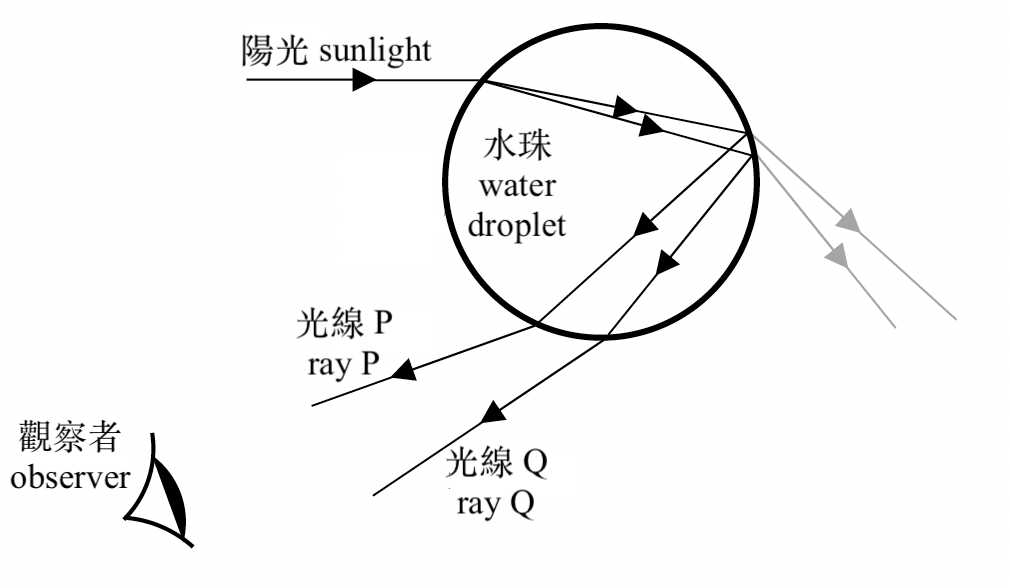
\includegraphics[width=0.6\linewidth]{1dn09idn093.png}\par}
        彩虹是一種特殊的光學現象。
        在某些天氣下,空氣中充滿水珠。由於水對藍光的折射率略高於紅光,又考慮到陽
        光由多種顏色的光線組成,入射水珠的陽光便會因折射而分散成可見光譜。這些光
        線在水珠中再經過一次反射和一次折射後,便會以可見光譜的狀態離開水珠。離開
        水珠後,當各種顏色的光線由不同角度抵達觀測者的眼睛時,觀測者便會見到彩虹。\\A rainbow is a special optical phenomenon. In certain weather conditions, the air is filled with water droplets. Due to the slightly higher refractive index of water for blue light compared to red light, and considering that sunlight is composed of various colors of light, the incident sunlight on the water droplets will be dispersed into a visible spectrum due to refraction. These rays of light undergo reflection and refraction once more within the water droplets before exiting in the form of a visible spectrum. When the rays of light of different colors reach the observer's eyes at different angles after leaving the water droplets, the observer will see a rainbow.
    \end{tcolorbox}\medskip
    圖(a)有助理解彩虹中的光學。若水珠是球形,則光線在水珠表面發生的折射和反射時的法
    線就是水珠的半徑(如虛線所示)。對於這種單色光而言,可取水的折射率為1.33。
    \\圖(b)則顯示了光線的總偏轉角 $\varphi$,$\varphi$ 的值等於兩次折射和一次反射,共三次偏轉中,各次的偏轉角度的總和。\\Figure (a) helps to understand the optics of a rainbow. If the water droplet is spherical, then the normal to the surface of the droplet during refraction and reflection of the light rays is along the radius of the droplet (as shown by the dashed line). For monochromatic light, we can assume the refractive index of water to be 1.33.
    \\Figure (b) illustrates the total deviation angle, denoted by $\varphi$. The value of $\varphi$ is equal to the sum of the deviation angles in each of the three instances: two refractions and one reflection.
        {\par\centering
            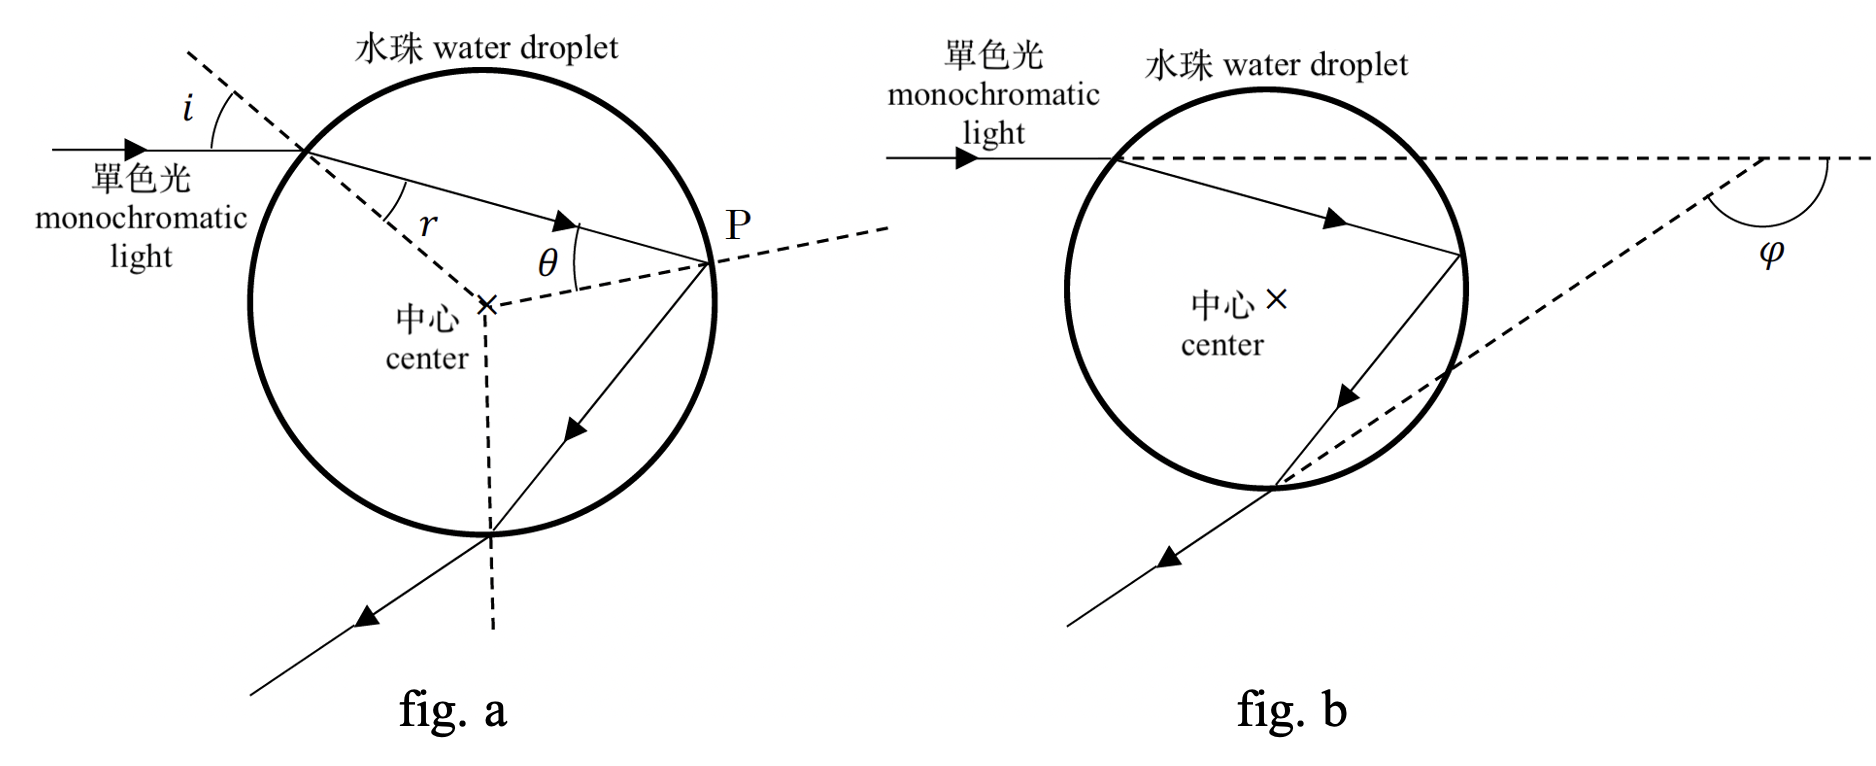
\includegraphics[width=.9\linewidth]{waterdropletsge.png}
            \par}\bigskip
    \clearpage
    \begin{parts}
        \part 解釋圖(a)中的光線P應是藍光還是紅光。\\Explain whether the light ray P in Figure (a) is blue light or red light.\zh{2}
        \dlines{2}
        \part 圖(b)中,$i$ = \dg{59.6}。\\In Figure (b), $i$ = \dg{59.6}.
        \begin{subparts}
            \subpart 求$r$的值。\\Find the magnitude of $r$.\zh{2}
            \dlines{2}
            \subpart 寫出 $\theta$ 的值,並解釋光線在P點會否發生全內反射。\\Write down the value of $\theta$, and explain whether total internal reflection occurs for light ray at P.\zh{3}
            \dlines{3}
            \clearpage
            \subpart 寫出這情況對應的總偏轉角 $\varphi$ 的值,並解釋彩虹出現時應面向還是背向太陽。\\Write down the value of the total angle of deviation $\varphi$ corresponding to this situation, and explain whether the rainbow should appear facing towards or away from the sun.\zh{3}
            \dlines{3}
        \end{subparts}
        \part 一個觀測者看到彩虹。對該觀測者而言,彩虹頂端的仰角是 \dg{30}。若他向彩虹方向前進數十米,彩虹頂端的仰角應大於、小於還是等於\dg{30}?解釋你的答案。\\An observer sees a rainbow. For this observer, the elevation angle of the top of the rainbow is \dg{30}. If the observer moves several tens of meters towards the direction of the rainbow, should the elevation angle of the top of the rainbow be greater than, less than, or equal to \dg{30}? Explain your answer.\zh{2}
        \dlines{2}
    \end{parts}
}{
}

\newprob{lq2}{
    一束藍光光束B射進一個透明的矩形塑膠塊PQRS,如圖中所示。
    已知入射角是\dg{70},玻璃對藍光的折射率是1.38。\\A blue light ray is incident onto a transparent rectangular plastic block PQRS, as shown in diagram. Given that angle of incidence is \dg{70}, and refractive index of plastic for blue light is 1.38.
    \bigskip
    {\par\centering
        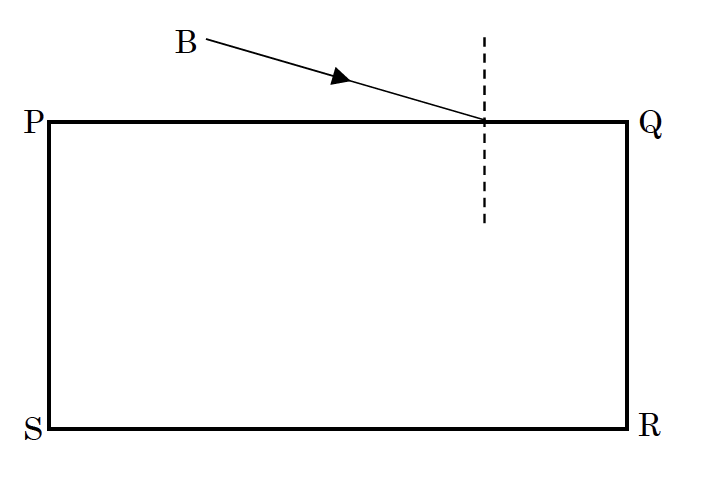
\includegraphics[width=0.5\linewidth]{8jx19m8enc8ecge.png}
        \par}
    \begin{parts}
        \bigskip
        \part 計算藍光光束B進入塑膠塊後,抵達QR邊時的入射角。\\Calculate the angle of incidence of blue ray B when it reaches the side QR inside the plastic block.\par\zh{3}
        \dlines{3}
        \clearpage\part 計算藍光光束B在塑膠塊的臨界角。\\Calculate the critical angle of blue ray B inside the plastic block. \zh{1}
        \dlines{1}
        \part 已知紅光在此塑膠塊中的速率是\vel{2.22e8},求塑膠塊對紅光的折射率。\\It is known that the speed of red light inside plastic block is \vel{2.22e8}, find the refractive index of plastic for red light.\zh{1}
        \dlines{1}
        \part 現把光束B換成白光。在上圖中畫出紅光和藍光進入PQRS至離開PQRS的光路。\\Now replace ray B with white light. Draw in the above figure the ray paths of red and blue rays as they enter and leave PQRS.\zh{3}
    \end{parts}
}{
    \textbf{Solution:}
    \begin{tasks}
        \task [(a)] $1.38\sin\theta=\sin70^\circ$
        \task [] $\theta=42.9^\circ$
        \task [] 入射角incident angle $=90^\circ-42.9^\circ=47.1^\circ$
    \end{tasks}
    \begin{tasks}
        \task [(b)] $1.38\sin\theta=(1)\sin90^\circ$
        \task [] $\sin\theta=\dfrac{1}{1.38}$
        \task [] $\theta=\sin^{-1}\left(\dfrac{1}{1.38}\right)=46.4^\circ$
    \end{tasks}
    \begin{tasks}
        \task [(c)] $n=\dfrac{\num{3e8}}{\num{2.22e8}}=1.35$
    \end{tasks}
    \begin{tasks}
        \task [(d)]
    \end{tasks}
}

\newprob{mc1}{
    一束由紅光和紫光組成的光線,射向矩形玻璃 塊。以下哪圖最能表示,光線通過玻璃塊的路徑?\\A ray consists of red and violet light, Which of the following best shows the paths of the ray through n rectangular block?
    \begin{tasks}(2)

        \task
        \topalign{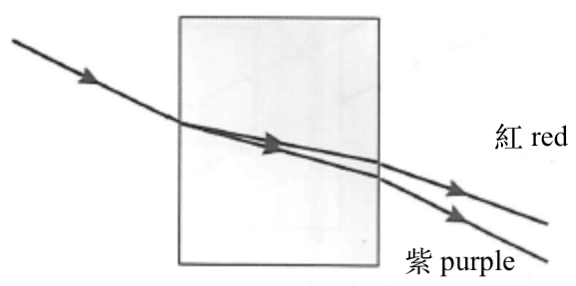
\includegraphics[width=0.8\linewidth]{d21d1d017.png}}
        \task
        \topalign{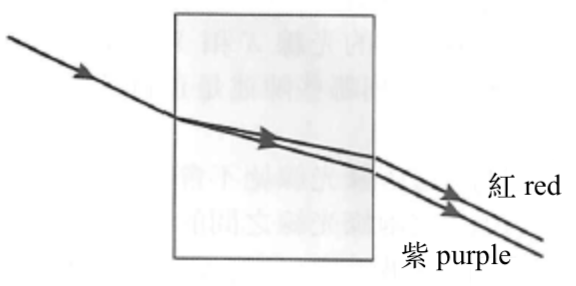
\includegraphics[width=0.8\linewidth]{xn98eu9e29n332f.png}}
        \task
        \topalign{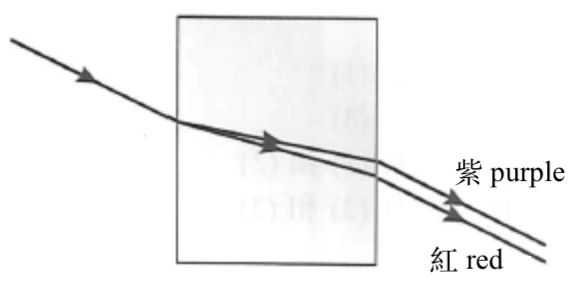
\includegraphics[width=0.8\linewidth]{dn0xu9dn23.png}}
        \task
        \topalign{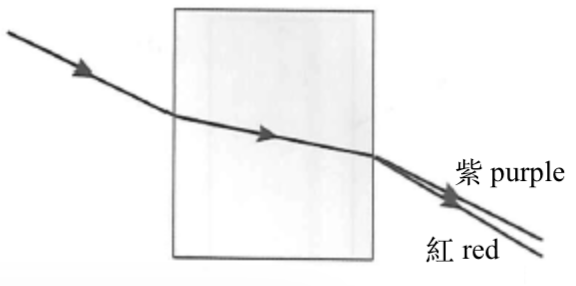
\includegraphics[width=0.8\linewidth]{x8un892.png}}

    \end{tasks}
}{}

\newprob{mc2}{
光線X從空氣沿法線射向玻璃三稜鏡 ABC,如上 圖所示。若整個裝置浸在水中,將會出現什麼結果?\\A ray of light X travels in air and strikes a glass prism ABC normally as shown above. What happens if the setup is immersed in water?
{\par\centering
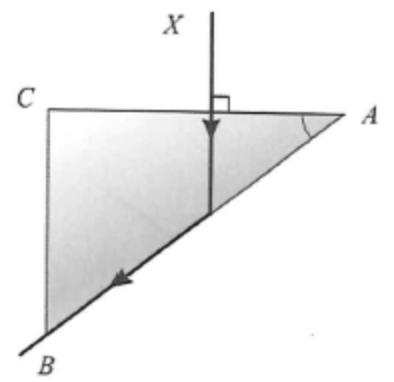
\includegraphics[width=0.25\linewidth]{xeu98neu32e3.png}\par}
\begin{tasks}
    \task 光線將在棱鏡內發生全內反射,然後 從 BC上某點離開。\\The ray will undergo total internal reflection inside the prism and then emerge from a point on BC.
    \task 光線將直線穿過 AB 而不會改變方向。\\The ray will pass straight through AB without change in direction.
    \task 光線將通過 AB 並偏折,在左邊射出。\\The ray will pass through AB and bend to the left side.
    \task 光線將通過 AB並偏折,在右邊射出。\\The ray will pass through AB and bend to the right side.
\end{tasks}
}{}

\newprob{mc3}{
    \topalignc{\par\centering
        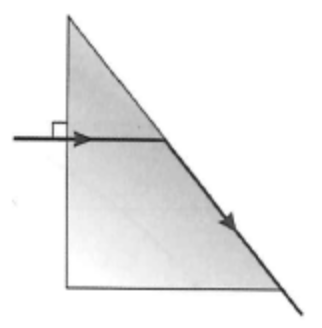
\includegraphics[width=0.25\linewidth]{d89q98ndwq.png}\par}\par
    一束窄的紅光,沿法線射向玻璃三棱鏡,然後 離開,如上圖所示。若以紫光取代紅光,下列 哪圖最能代表光束新的路徑?\\A narrow beam of red light strikes a triangular glass prism normally and emerges as shown above. If the beam is replaced by violet light, which of the following diagrams best represents the path of light?
    \begin{tasks}(2)
        \task
        \topalign{\par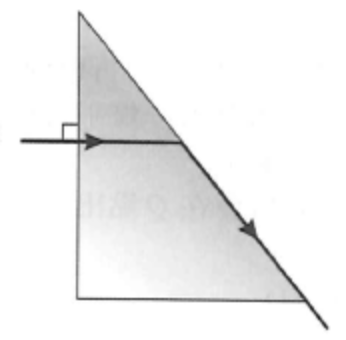
\includegraphics[width=0.6\linewidth]{und89wqudage.png}\par}


        \task
        \topalign{\par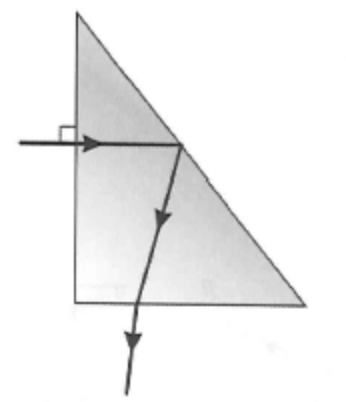
\includegraphics[width=0.6\linewidth]{djioqwge.png}\par}


        \task
        \topalign{\par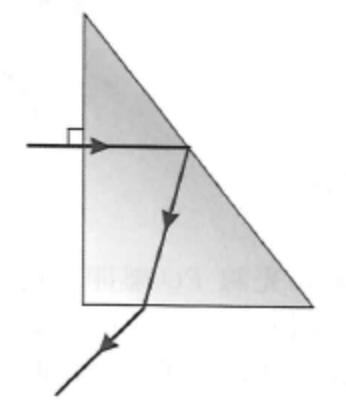
\includegraphics[width=0.6\linewidth]{diqwdoiqw2.png}\par}


        \task
        \topalign{\par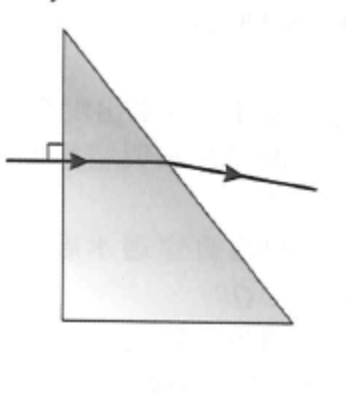
\includegraphics[width=0.6\linewidth]{dwq1d1dcddd13.png}\par}


    \end{tasks}
}{}
\newprob{mc4}{
    \topalignc{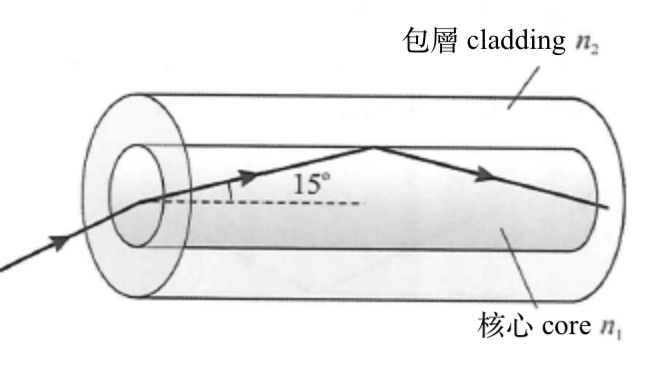
\includegraphics[width=0.5\linewidth]{d2nuc9u8293uc2nr23.png}}
    光導纖維的玻璃核芯(折射率 $n_1$)以包層(折 射率 $n_2$)包裹著。上圖顯示一條光線從空氣進 入玻璃核心,並經過一次全內反射。下列哪些 陳述是正確的?\\The glass core (refractive index $n_1$) of an optical fibre is surrounding by a cladding (refractive index $n_2$). The diagram shows how a ray of light enters into the glass core and then undergoes total internal reflection. Which of the following statements is/are true?
    \begin{statements}
        \task 玻璃核心和包層之間的臨界角大於 \dg{75}。\\The critical angle between the glass core and the cladding is greater than \dg{75}.
        \task $n_1>n_2$
        \task $n_1>\dfrac{1}{\sin 75^\circ}$
    \end{statements}
    \begin{tasks}
        \task 只有(1) \tab\tab (1) only
        \task 只有(3) \tab\tab (3) only
        \task 只有(1)和(2) \tab\tab (1) and (2) only
        \task 只有(2)和(3) \tab\tab (2) and (3) only
    \end{tasks}
}{}
\newprob{mc5}{
    \topalignc{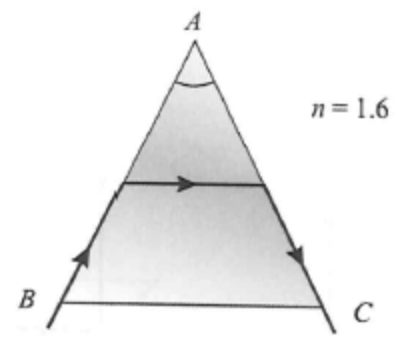
\includegraphics[width=0.3\linewidth]{x98nu823.png}}\par
    三棱鏡 ABC 所用材料的折射率為1.6。一條 光線沿棱鏡的一面入射,並沿棱鏡的另一面離 開,如上圖所示。棱鏡上的角A 是多少?\\A triangular prism ABC is made of material of refractive index 1.6. A ray of light at glancing incidence leaves the prism also at glancing angle as shown. What is the angle A of the prism?
    \begin{tasks}
        \task \dg{39}
        \task \dg{56}
        \task \dg{65}
        \task \dg{77}
    \end{tasks}

}{D}
\newprob{mc6}{
    \topalignc{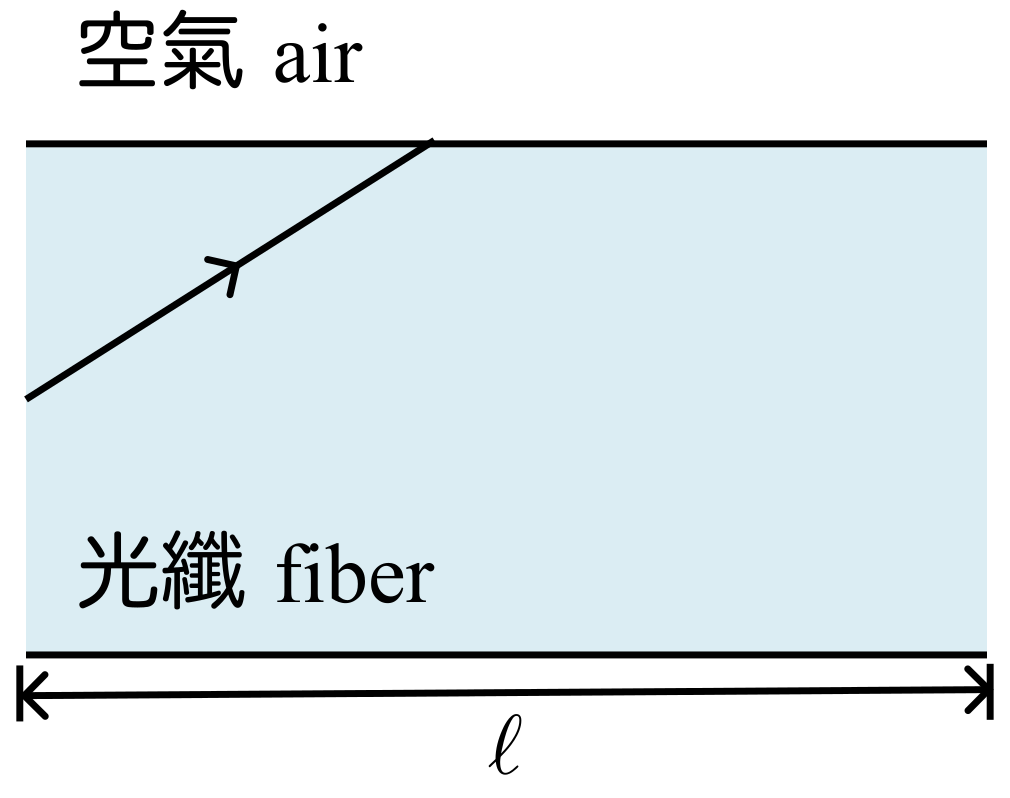
\includegraphics[width=0.3\linewidth]{dqwijqwoe.png}}
    一條光線沿筆直的光纖傳播。已知光纖長度為 $\ell$,折射率為 $n$。光線從光纖一端傳播至另一端 的最短及最長時間分別是多少?設$c$為光在真空 中的速率。\\A light ray travels in a straight fibre of refractive index $n$ and length $\ell$. What are the min. and max. time required for the light to travel from one end of the fibre to the other end without any light leak? ($c$: speed of light in vacuum)
    \begin{tasks}
        \task [] 最短時間min. time\tab 最長時間max. time
        \task $\dfrac{\ell}{nc}$\tab\tab $\dfrac{n\ell}{c}$
        \task $\dfrac{\ell}{nc}$\tab\tab $\dfrac{n^2\ell}{c}$
        \task $\dfrac{n\ell}{c}$\tab\tab $\dfrac{n^2\ell}{c}$
        \task $\dfrac{n\ell}{c}$\tab\tab $\dfrac{n^4\ell}{c}$
    \end{tasks}
}{C}
\newprob{mc7}{
    \topalignc{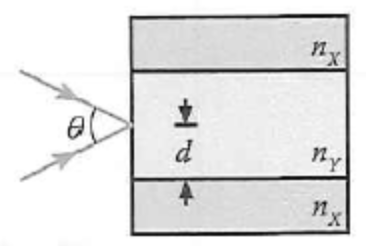
\includegraphics[width=0.25\linewidth]{d9i09n293d.png}}\medskip
    \par 一條纖維由包層(折射率 $n_X$)及核心(折射率 $n_Y$)組 成。光線在圖中所示、頂 角為$\theta$的圓錐範圍內射入 纖維,便可透過全內反射 傳播至遠處。核心的半徑 為$d$,如圖。\\A fibre is made of a core (refractive index = $n_Y$) embedded in a cladding (refractive index = $n_X$). Its core has a radius $d$. Light rays within a cone of vertex angle $\theta$ at the central axis of the fibre can be guided through the fibre by total internal reflection.
    \par 要增加$\theta$的值,可以\\The angle $\theta$ can be increased by
    \begin{statements}
        \task 減少$d$的值。\\reducing d.
        \task 減少$n_X$的值。\\reducing $n_X$
        \task 減少$n_Y$的值。\\reducing $n_Y$
    \end{statements}
    \begin{tasks}
        \task 只有(2) \tab\tab (2) only
        \task 只有(3) \tab\tab (3) only
        \task 只有(1)和(2) \tab\tab (1) and (2) only
        \task 只有(1)和(3) \tab\tab (1) and (3) only
    \end{tasks}
}{A}

\newprob{mc8}{
一束光線投射至一塊長方形玻璃磚。玻璃磚闊度 為$w$,折射率為$n$。光線以角度$\theta$進入玻璃磚 後,產生旁向位移$d$,如圖。下列哪情況能增加 $d$的值?\\A rectangular glass block has a width $w$ and a refractive index $n$. When a light ray strikes it at an angle $\theta$ as shown, the emergent ray is laterally displaced by a distance $d$. In which of the following situations will the value of $d$ increase?
{\par\centering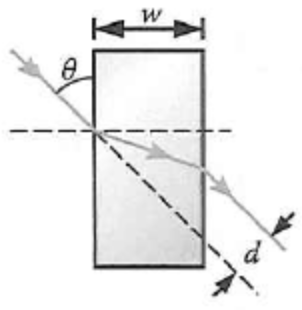
\includegraphics[width=0.22\linewidth]{8x9nu23.png}\par}
\begin{statements}
    \task 增加$n$ 的值 \\$n$ increases
        \task 增加$\theta$ 的值\\$\theta$ increases
        \task 增加$w$ 的值\\$w$ increases
\end{statements}
\begin{tasks}
    \task 只有(1)和(2) \tab\tab (1) and (2) only
    \task 只有(1)和(3) \tab\tab (1) and (3) only
    \task 只有(2)和(3) \tab\tab (2) and (3) only
    \task (1), (2) 和 (3)\tab\tab (1), (2) and (3)
\end{tasks}

}{B}